In the \cref{sec:c-lang}, I discussed how competing forces of inherited
portability requirements, proximity to hardware, and the desire for more
aggressive optimisations led to complex and subtle technical resolution by
stakeholders in the \kl{ISO} standard of C. I also mentioned that its nature as
a prose document, with natural language ambiguities and omissions, as well as
divergence C as used \kl{de facto}, mean that its semantics are unreasonable
for a human to adhere to, and challenging to build into tools directly,
without making some sort of simplifying assumptions.

Existing program logic frameworks for C such as Verifiable C~\sidecite{appelSF5}
and RefinedC~\sidecite{sammler2021refinedc} take the approach of building a
logic directly above an operational semantics for a language which is
recognisably C, minus some desugaring to consolidate similar constructs. They
attempt to retain as many C features (control flow, variable scoping, aliasing,
loose evaluation order, pointer manipulation rules) as possible, but make
simplifying assumptions where it would be impractical otherwise.

Given that \kl{CN}'s headline goal (\cref{sec:cn-intro}) is to work with
pre-existing C programs, which rely on many if not all of those impractical
features, adopting the conventional approach would quickly use up most of its
complexity budget and make the other goal (of reducing the expertise required
to do verification) unfeasible.

Instead, \kl{CN} builds directly upon the
\kl{Cerberus}~\sidecite{memarian2022cerberus} executable and empirically
validated semantics for C. Not only does \kl{CN} benefit from the
\emph{accurate} semantics for both \kl{ISO} and \kl{de facto} C, it benefits
most from the \emph{usability} of it. This is because, Cerberus is elaborated
into a relatively small calculus \emph{\kl{Core}}, which translates all of C's
complexity into a first-order functional language with a few special (but easy
to understand and specify) constructs.

Additionally, \kl{CN} is intended to be used more like a \emph{type system} in
an IDE than a program logic inside a proof assistant. Ideally, instead of
seeing intermediate goals in a sophisticated separation logic, and needing to
be well versed with a range of inference rules and automation tactics, a user
sees their C program, scattered with predictable and lightweight annotations in
comments, in an editor which either indicates success, or clear and helpful
error message.

Aside from the fact that the notion and mode of use of a type system is more
familiar to most programmers (an advantage not to be scoffed at), this approach
also allows \kl{CN} to use and advance the extant literature on building
refinement type systems on top of existing languages.

This type system approach also leads to other desiderata and their
corresponding responses. If we want to follow a type system approach, we want
to minimise obvious annotations and justify why the necessary ones are so, we
need to track carefully the flow of information in the type system, using a
\kl{bidirectional} approach. We also need some sort of automation so as to not
burden the programmer with proving things like $1 + 1 = 2$. Similar to
VeriFast~\sidecite{jacobs2011verifast} and Frama-C\sidecite{kirchner2015frama},
\kl{CN} enlists the support of SMT solvers to mitigate this. When trying to
verify code against expressive specifications, this could lead to
non-termination, so \kl{CN} also restricts the expressiveness of the assertion
language, and the queries it sends to the SMT solver. And given the importance
of managing resources in C, the typing discipline needs to be substructural.

The \kl{CN} assertion language syntax aims to be expressive enough to verify
real world C, but also restricted enough to limit the aforementioned technical
problems, and intuitive enough to a target audience of systems programmers who
happen to know Haskell (or Rust).

With this many constraints and design decisions, it is easy to doubtful of the
elegance and feasibility of this approach, let alone consider proving such a
type system sound. As I will show in \nameref{chap:kernel-typing}, whilst the setup
might be novel, multi-faceted and large, the definitions are relatively
straightforward, and the proof of soundness can be done syntactically. Both the
definitions and the proof are modular with respect to the heap, so that
changing the memory object model does not require redoing the entire soundness
proof. The formalisation is close enough to the surface syntax of \kl{CN} so
that a correspondence between the two can be stated simply and precisely, and
close enough to the implementation to offer actionable insights.

\chapter{Formalisation Background}%
\label{chap:formal-background}

\margintoc{}

The components of \intro{Kernel CN} all have precedent in prior work; the main
new contribution is the adaptation and confluence of those ideas. This chapter
will set out \kl{CN}'s design goals and origins, recapitulate the disparate
concepts used in CN, and along the way discuss how they satisfy the
aforementioned design goals.

\section{\kl{CN} design goals and constraints}%
\label{sec:cn-goals}

Aiming for \emph{``a verification tool whose aspirational goal is to lower the
cost of C verification from a Rocq programmer who knows separation logic to a
systems programmer who knows Haskell''} (\cref{sec:cn-intro}) helps narrow
down the large design space of verification tools.

The reason for picking this particular goal is in \kl{CN}'s origins as
an attempt to verify the pKVM hypervisor, developed by Google.

Before I explain pKVM, I need to explain the context for this. The Android
operating system runs on billions of devices worldwide, playing a central role
in many lives, including handling an enormous amount of sensitive data. This
means that security is paramount, however because each device runs its own
kernel (up to half the code is not Android's version of Linux), updates are
very challenging and expensive to test and deploy to each device. Aside from
security issues, this also leads to fragmentation of Android, so devices and
apps are not all up-to-date and the long delay (at least 18 months) between
Linux and device releases makes to difficult upstream features and fixes.%
\sidenote{%
TODO\@: cite these properly.
\begin{itemize}
    \item \url{https://youtu.be/7novnkldMmQ?feature=shared}
    \item \url{https://youtu.be/wY-u6n75iXc?feature=shared} and \url{https://lwn.net/Articles/836693/}
    \item \url{https://source.android.com/docs/core/architecture/kernel/generic-kernel-image}
    \item \url{https://source.android.com/docs/core/virtualization/whyavf}
    \item \url{https://googleprojectzero.blogspot.com/2020/02/mitigations-are-attack-surface-too.html}
    \item \url{https://lpc.events/event/7/contributions/780/}
\end{itemize}
}

Whilst some of this has been mitigated with the introduction of
\intro[GKI]{Generic Kernel Images (GKI)}, which provide a small and stable
kernel ABI \emph{for a particular long-term release} version of Android, there
are still security issues present in this model, because the kernel is too
large (20 million lines of code) to be a reasonable trusted computing base, and
the drivers vendors ship with a device are part of it.

Some manufacturers use hypervisors, which attempt to isolate the kernel from
the rest of the system by running Android and other hardware components in
virtual machines, such `secure' parts of the device storing sensitive data.
Aside from security, hypervisors are also used to partition memory at boot-time
so that devices can use it for things like direct memory access, and run
arbitrary code outside of Android, which is worrying because this code would
run at a more privileged level than Android itself. All of this just
\emph{shifts} the attack surface, and has also resulted in \emph{more}
fragmentation at the hypervisor layer.

Similar to GKI, the proposed solution to standardise the hypervisor used. There
is already a mature hypervisor which is part of the Linux kernel, the
Kernel-based Virtual Machine (KVM)\@. It is set up so that a host kernel can
dynamically allocate virtual machines for guests to run on, and protect the
host from the guests. However, at the start of the project, the API exposed by
the hypervisor to the host kernel offered too much control, and guests were not
protected from the \emph{host}. This is a problem because the guest could be
running code for a secure hardware component (e.g.\ a biometric authenticator),
the host could be a compromised version of Android, so an attacker could still
get access to sensitive information.

To solve this, Google, as part of the Android Virtualisation Framework, is
developing a \intro[pKVM]{protected KVM (pKVM)}, which runs \emph{underneath}
the kernel, and ships \emph{as part} of the kernel image. Not only does this
tight coupling remove issues around ABI compatibility between the hypervisor
and the kernel, since the source is always in the same repository, it also
allows pKVM to commit to only handling implementing a select few functions such
as virtual memory management and remain very small, and rely on the Linux
kernel to manage the rest, such as scheduling, device drivers and power
management.

If successful, this could make the attack surface a lot smaller, but it could
also make it one that is used very widely. It is in this context that Google
sought assistance from the research community to see if verifying the kernel
was feasible, \emph{on an ongoing basis}. A one-and-done verification of pKVM
which takes an army of PhD students and postdocs a few years to verify and is
years out of date by the time is developed is not worth the investment, a
tool which C kernel hackers can understand, use and maintain proofs as they
make changes to very important security critical code is.

So not only does this background explain \kl{CN}'s headline goal, it also
clarifies some of the \emph{constraints} on its design:
\begin{itemize}
    \item Because kernel hackers wrote the code, and are intending to use
        conventional compilers to build and run it,\sidenote{Assuming the
        binary can be verified as well, perhaps with input from \kl{CN}.} we
        cannot rely on (hopefully sound) approximation to the semantics of C
        \textemdash{} we want and need something that matches and can handle
        its real world behaviour as closely as possible.
    \item Because it will be used by kernel hackers, we want a story that is
        is accessible and acceptable to them. These are very smart and
        capable people, who do not have the time or support to get up to
        speed with separation logics and interactive proof assistants, or be
        amenable to change their (or more importantly, their organisations)
        workflows substantially. A ``fancier type system'' which runs as part of
        the \intro[CI]{continuous integration (CI)} pipeline is much more
        likely to be used and adopted in this context.
    \item Similarly, because the annotations will be read by kernel hackers,
        and upstreamed into Linux, we want them to be minimal and relatively
        easy to understand. Not only does this affect the design of the type
        system to manage the flow of information carefully, this encourages
        exploring how best to automate as many obvious things as feasible.
\end{itemize}

In turn, these constraints feed into concrete technical choices which \kl{CN}
makes:
\begin{itemize}
    \item To capture real-word C behaviour, \kl{CN} uses the \kl{Cerberus}
        empirically validated semantics.
    \item To integrate into existing workflows, \kl{CN} appears to users
        as a fancy type system.
    \item To retrofit the type system on top of existing ones, and in
	particular to ensure erasure, \kl{CN}'s type system uses
	\intro{refinement types}.
    \item To automate proofs of constraints, \kl{CN} relies on SMT solvers.
    \item To ensure decidability (termination), and aim for reasonable in
        practice performance, \kl{CN} follows a \emph{liquid} typing
	discipline, restricting the queries it sends to the SMT solver.
    \item To minimise constraint annotations, \kl{CN}'s type system is
        formalised and implemented in a \kl{bidirectional} style.
    \item To check the resource management of C programs, \kl{CN}'s type
        system uses \intro{linear} types, using the grammar of separation
        logic assertions.
    \item To stay within the \kl{liquid} typing discipline \emph{and} avoid
	quantifier instantiation annotations, \kl{CN} uses precise assertions
	with a \kl{mode}d disciple for predicate arguments.
    \item To make such precise assertions with a mode discipline easier to read,
	write and explain, \kl{CN} presents users with \emph{monadic} syntax.
\end{itemize}

\section{Cerberus and Core for an usable and accurate C semantics}%
\label{sec:cerberus-core}

\intro{Cerberus} is an empirically validated and executable semantics for
\kl{ISO} and \kl{de facto} C, specifically C11. A detailed comparison
between it and other C semantics is available in the Related Work chapter
of \sidetextcite{memarian2022cerberus}, but for the purposes of \kl{CN},
it suffices to say it captures real-world C.

Where \kl{Cerberus} really shines with respect to \kl{CN}'s use case in
\emph{how} it captures this executable semantics. In particular, it does so by
\emph{compositional elaboration} into a \emph{relatively simple first-order
functional language}, unlike other semantics, which are defined over some
desugared and consolidated grammar closely resembling C.

This approach drastically simplifies many tricky parts of C. For example,
\cref{fig:perplexing-ub} is accepted by the frontend, complete with strange
scoping and strange control flow which jumps \emph{into} a loop body. And in
this particular program, the fact that the \emph{mutable variables} \cinline{x}
and \cinline{*p} alias, or the myriad of \kl[UB]{undefined} or \kl{unspecified}
behaviours programmers might usually be familiar with, is not the reason it is
illegal, but due to subtle rules around block scopes and variable
initialisation. The way Cerberus does this is by making explicit C features
such as \kl{UB}, \kl{unspecified} or implementation-defined behaviours,
coercions, loose evaluation order and so on.

\begin{marginfigure}
    \cfile[breaklines]{code/perplexing-ub.c}
    \caption{This example has undefined behaviour because of the subtle
        interaction between block scopes, variable initialisation and
        \cinline{goto} statements in C. But, if the comment is uncommented,
        then the program has defined behaviour.}\label{fig:perplexing-ub}
\end{marginfigure}

Instead of working directly over something similar to C and trying to express
static and dynamic semantics over something so complex, \kl{Cerberus}
elaborates C into \intro{Core}, a not-too-large calculus where each construct
is designed to capture some peculiarity of C. It is split into two fragments, a
pure (\cref{fig:pure-core-grammar}) and effectful
(\cref{fig:effectful-core-grammar}) which embeds the pure one.

The pure fragment is pure in the sense that it allows no memory operations, but does
include the effect of undefined behaviour explicitly with the
\coreinline{undef()} operator. This aspect of the language handles % chktex 36
things like implicit type conversions or bounded arithmetic. As visible from the
grammar, the pure part is very much a first-order functional language with
recursive functions with some constructs specific to C such as pointer
arithmetic on arrays and struct fields, structs, unions and
specified/unspecified/integer values.

\begin{figure*}[tp]
    \ContinuedFloat*
    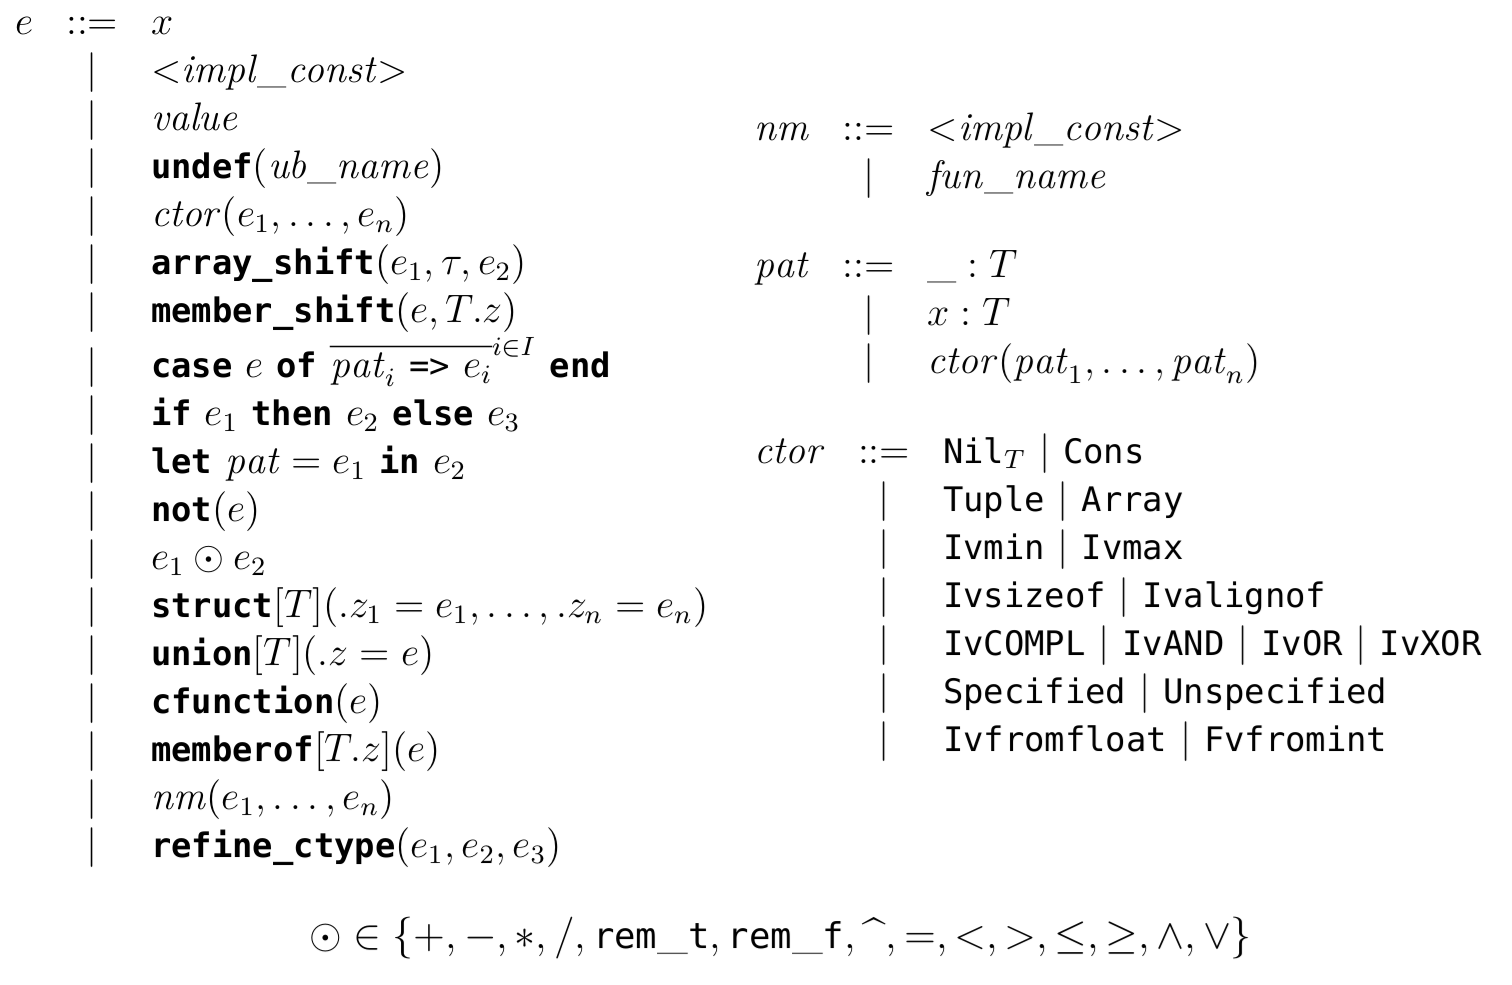
\includegraphics{figures/pure-core.png}
    \caption{The pure fragment of Core.}\label{fig:pure-core-grammar}
\end{figure*}

The effectful fragment captures interactions with memory (via a memory
interface), various ordering constraints, and more exotic control flow with a
goto-like operator used in the elaboration of C's iteration and \cinline{goto}
statements. The distinction between the pure and effectful fragments is is in
fact unrelated to the distinction between expressions and statements in C,
since both are elaborated into effectful expressions (for example,
\coreinline{PtrEq} which tests for for pointer equality).

I will discuss \coreinline{memop()} in more detail in % chktex 36
\nameref{chap:mem-model-explained}. For now it suffices to say that the
operations are effects, part of the memory interface \kl{Core} uses to abstract
over choices of different handlers, implementations of those effects in a
specific memory object model.

The following constructs are all related to evaluation order:
\coreinline{neg()}, \coreinline{unseq()}, \coreinline{let weak}, % chktex 36
\coreinline{let strong}, \coreinline{bound()}, \coreinline{nd()}, % chktex 36
\coreinline{par()}. These were supported in the implementation at one % chktex 36
point,\sidenote{See note~\ref{sn:new-inf}.} but stopped working due to a change
in the resource inference scheme, and not enough of a priority to re-enable. I
did not attempt to formalise their complex operational behaviour;
I considered supporting these constructs using fractional permissions,
but decided to leave that for future work because of the noise and complexity
it would add to the initial version of the formalisation.

The \coreinline{ccall()} and \coreinline{pcall()} constructs for calling % chktex 36
elaborate C functions and Core procedures (effectful functions) respectively.
They differ only in how the name of the procedure to be called is found, with
\coreinline{ccall()} using the memory interface to do so. % chktex 36

The \coreinline{save()} operator is \kl{Core}'s way of introducing named % chktex 36
continuations with default arguments. The label $l$ and arguments $x_1, \ldots,
x_n$ are in scope in $E$; those variables are associated pure expressions
provided by the \coreinline{run()} operator or with the default $e_1, \ldots, % chktex 36
e_n$ otherwise if the operator is reached otherwise. This is the \cinline{goto}-like
operator referred to earlier, which is used to elaborate all of C's iteration
and \cinline{goto} statements.

The important aspect from our purposes is that while control flows into
\coreinline{ccall()}, \coreinline{pcall()} and \coreinline{run()}, it % chktex 36
only returns from the first two and not the last.

\begin{figure*}[tp]
    \ContinuedFloat{}
    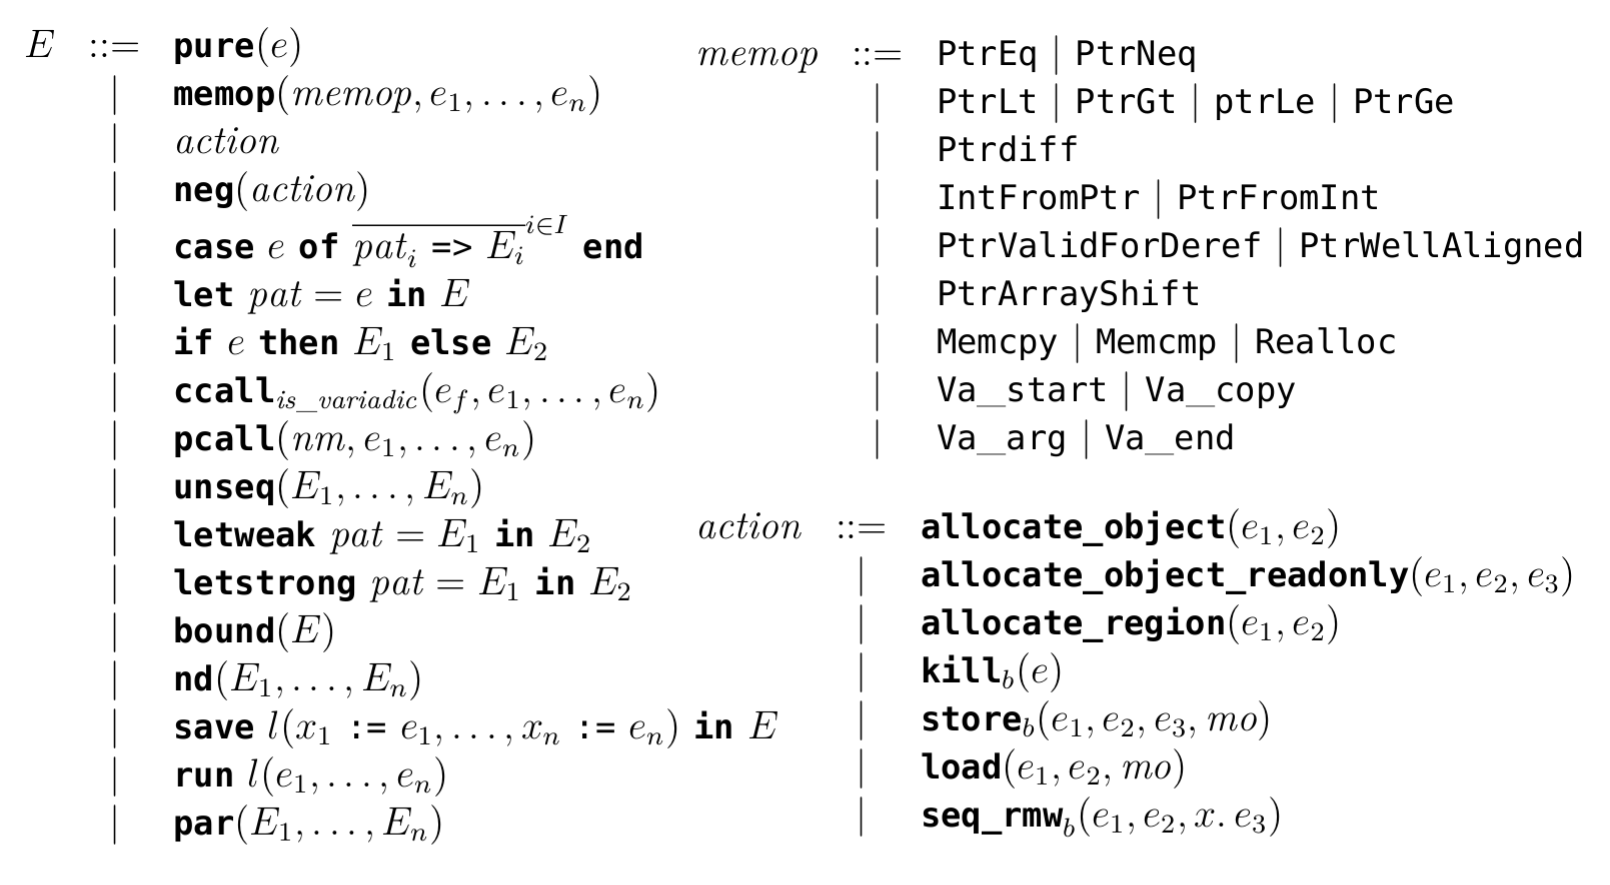
\includegraphics{figures/effectful-core.png}
    \caption{The effectful fragment of Core.}\label{fig:effectful-core-grammar}
\end{figure*}

We can see an example of Cerberus' elaboration into \kl{Core}, by recalling the
linked integer list append function from \cref{fig:append-c}, reproduced
in \cref{fig:append-c-formal} for convenience.

\begin{marginfigure}
    \centering
    \cfile[breaklines]{code/append_plain.c}
    \caption{Linked integer list append in C.}\label{fig:append-c-formal}
\end{marginfigure}%

\begin{figure*}[p]
    \centering
    \begin{minipage}{1.2\textwidth}
        \corefile{code/append_plain.core}
    \end{minipage}
    \caption{Elaboration of linked int list append in C into
        \kl{Cerberus} \kl{Core}; library functions and \cinline{else}-branch
        omitted.}\label{fig:append-core}
\end{figure*}%

The elaboration is presented in \cref{fig:append-core}. To save space,
definitions the \kl{Core} standard library are omitted, as are choices about
implementation-defined details and the elaboration of the
\cinline{else}-branch. A few things are note-worthy:
\begin{itemize}
    \item The translation is \intro{compositional}. Each function, block,
        statement and expression is elaborated in isolation, based only
        on its parts, and follows the structure of the original C program.
    \item Each variable function argument and local gets its own storage via the
        \coreinline{create} function. Reads, writes, and de-allocations are
        represented with \coreinline{load}, \coreinline{store},
        \coreinline{kill} respectively.
    \item Loose evaluation order (for example between the expressions of a \cinline{==})
        are represented using \coreinline{unseq} and \coreinline{let weak} constructs.
    \item UB is made explicit in the syntax of the program, for example if \cinline{xs} was
        an unspecified pointer value (line 23) or if the function exited without a return statement
        and its `return value' was used elsewhere (line 71).
\end{itemize}

In particular, \kl{compositional}ity is just as important, if not more, than the
target language being a first-order functional language with effects. Given
that we want users to annotate programs at the C level, if we wish to type
check \kl{Core}, we need to be able to transport those annotations through the
elaboration process too, and place them at the appropriate program points.

If \kl{Cerberus} were to have elaborated into a dataflow graph instead of \kl{Core},
such transporting would be a major undertaking in itself. It might achievable
for function pre- and postconditions, but would become much more challenging
for loops, and \coreinline{goto} and even between specific statement as proof
hints to \kl{CN}. With a \kl{compositional} mapping, placing annotations
structurally, and relating annotations mentioning C variables to \kl{Core}
variables becomes feasible.

In principle, the compositional mapping also ensures that errors in \kl{Core}
elaboration can be related back to useful source locations in the original C
program. However, in practice, though \emph{compositional}ity does
\emph{enable} this, it requires a good amount of engineering effort to
accomplish (\cref{sec:error-msgs}). Another challenge is that though
elaboration simplifies greatly the checked language, it also increases the
distance between the checked and the typed language, which is felt acutely when
attempting to relate failures in SMT queries back to what users wrote,
particularly when those SMT are part of an inference procedure, rather checking
C source assertions (\cref{sec:counter-ex}).

\section{Decidable refinements for retrofitting and counter-examples}

\kl{Core} already has a straightforward \kl{bidirectional} type system as a
sanity check on the output of elaboration. It has not been used for a
rudimentary proof of soundness with respect to the dynamic semantics, since
such a theorem would be just another sanity check (on the dynamic semantics).

\begin{marginfigure}
    \centering
    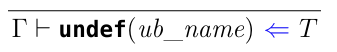
\includegraphics{figures/core-ub-typing}
    \caption{Typing rule for the \coreinline{undef()} pure expression as % chktex 36
        mentioned in \textcite{memarian2022cerberus}. The type system is set up
        in a \kl{bidirectional} way, with checking judgements represented by
        $\color{blue}{\Leftarrow}$, and synthesis with
        $\color{red}{\Rightarrow}$.}\label{fig:core-ub-typing}
\end{marginfigure}

This is evidenced by the typing rule for \coreinline{undef()} % chktex 36
(\cref{fig:core-ub-typing}). Since \kl{UB} is by definition, assumed to be
absent in a valid C program, the type system must accept any type as validly
checking against \coreinline{undef()}. % chktex 36

At a minimum, to prove C programs safe, what we would like is a type system
expressive enough to \emph{prove} the absence of \kl{UB}. If the type checking
context is enriched to track the control flow path to reach this point in the
program, for example by tracking conditions (or their negations), then the
typing rule for \coreinline{undef()} would simply require that the context % chktex 36
be inconsistent, i.e.\ able to prove false. To illustrate this point with
a trivial example, consider the nested \mintinline{py}{if} statements in
\cref{fig:dead-code}.

\begin{marginfigure}
    \inputminted[breaklines,mathescape,fontsize=\small]{py}{code/dead_code.py}
    \caption{A contrived example on how tracking control flow assumptions
        within a program could be used to prove the impossibility of
        undesirable behaviour.}\label{fig:dead-code}
\end{marginfigure}

Since we know from the outer \mintinline{py}{if} that \mintinline{py}{x} is
greater than or equal to 5, the check for \mintinline{py}{x} being strictly
less than 4 is always going to evaluate to \mintinline{py}{False} and so go to
the \mintinline{py}{else} branch rather than raise the exception. When tracking
constraints, this unreachability or dead code is represented by an inconsistent
context, from which we can prove $\mathsf{false}$.

In general, to express and track these constraints in types, we need to be able
to talk about computational variables and values \emph{at the type level},
introducing a form of dependency. However, because we do not want to change the
programming language whose type system we are enriching (such as in a
\kl{dependent type} system) we are not adding the ability for computation to
depend on types, so we retain the property of recovering the original program
and dynamic semantics after erasing the expressive types we fit on top of them.

This approach of enriching the expressiveness of types on an existing language
whilst retaining the erasure is known as \intro{refinement types}. There is a
rich history of the origins, naming and development of these
ideas,~\sidecite{jhala2021refinement} and so I will focus only on the strands
relevant to \kl{CN}.

If our goal is to minimise annotations and not require proofs for obvious
statements, then we need some sort of automation to dispatch proof
obligations.\sidenote{Recall the examples shown in
\cref{fig:call-incr,fig:call-incr-fail}, where \kl{CN} deduces
\cinline[breaklines]{y <= MAXi32()} from the constraint \cinline[breaklines]{y
<= 100i32}.} However, once we have rich constraints being tracked by the type
system, we have a first-order logic with arithmetic and so skirt close to
undecidability for the type system. There are type system for real-world
programming languages (such as Hack or F$^*$) which are undecidable, and so
could just never terminate on some code, but have automation which works fine
in practice, so why does this point require any special consideration?

Aside from the pleasing theoretical property of having a decidable type system,
or having to tell users ``just increase the timeout'',  there are a couple of
factors which lean us in this direction, namely to be able to use SMT solvers
in a \emph{fast} and \emph{predictable} manner. Recognising that whilst
decidability can still technically mean exponential, or very often, NP-complete
complexity for problems does not negate the empirical observation that in
practice, decidable theories tend to be quite fast, and their speed (and
solvability) much less susceptible to heuristics being triggered. It is a proxy
for performance, albeit an imperfect one.

It also helps that the size of SMT problems generated by type checking
\emph{tend} to be reasonably small, at least compared to the sorts of problems
which SMT solvers are typically used for, because the amount of code humans
write between annotations is limited by cognitive capacity (and hopefully,
diligent code reviewers).

\kl{CN} ensures decidability by following restrictions on quantifiers as set
out by the liquid types~\sidecite{rondon2008liquid} approach. In practice, this
means ensuring that the constraints sent to the SMT solver are free of
quantifiers. When this approach is insufficiently expressive, \kl{CN} offers a
lemma mechanism to export and prove claims in the \kl{Rocq} interactive proof
assistant.

Aiming for decidability also has the added benefit of extracting a concrete
\kl{counter-example} (see \cref{sec:counter-ex}), which is used to explain
constraint failures in terms of concrete values for \kl{Core} program variables
(a subset of which correspond to C program variables).

\section{Bidirectionality for taming subtyping}\label{sec:bidir-subtyping}

Using a liquid typing discipline automates away the problem of tedious proof
obligations with calls to an SMT solver, but introduces the new of \emph{when}
during type checking is the right time to use it? This is because implications
induces a subtyping relation in the type system, and so the question becomes:
when is the correct time to use the subsumption rule, as shown in
\cref{fig:subsumption}?

\begin{marginfigure}
  \begin{mathpar}
      \inferrule{\Gamma{} \vdash{} e \mathrel{{:}} \{ x \mid{} \phi{} (x) \}  \\ \phi(x) \Rightarrow{} \phi' (x) }
                {\Gamma{} \vdash{} e \mathrel{{:}} \{ x \mid{} \phi' (x) \}}
  \end{mathpar}
  \caption{Subsumption rule using for a system with subset types and logical
      implication $\Rightarrow$ as the subtyping relation.}\label{fig:subsumption}
\end{marginfigure}

% TODO fix the spacing around the curly braces with \,

Going back to the example in \cref{fig:dead-code}, let us imagine we are in a
type system where the contexts $\Gamma$ are either $\cdot$ or $\Gamma, \{ x \mid
\phi(x) \}$, where $\phi$ represents some constraint on $x$. In particular, we
are not accumulating control flow constraints in the context, only
in the variable's subset type. We would like to check that the function
\mintinline{py}{gt_zero} satisfies its postcondition. $ \{ \mathsf{ret} \mid
\mathsf{ret} > 0 \} $, i.e.\ it returns a value greater than 0 and does not
raise an exception.

Working forwards, we start off with a type for $\{ \mathsf{x} \mid \top \}$.
Inside the function, we are checking both branches because we cannot statically
rule one of them out. In the true case, we now \emph{refine} the type to $\{
\mathsf{x} \mid \mathsf{x} \geq 5 \}$. Because we are not sure when to apply
the subsumption rule, and we can apply it at any time, we apply it now, and
have $\{ \mathsf{x} \mid \mathsf{x} > 0 \}$, because $\mathsf{x} \geq 5
\Rightarrow \mathsf{x} > 0$. At this point, we cannot statically rule out the
either branch of the condition, so we start checking the one with the
exception, instead of skipping over it as dead code.

Whilst quite contrived, it illustrates the point that we would like some sort
of principled scheme to know when to use the subsumption rule, and with which
constraints. We could avoid this by requiring users annotate their code at
every step, but though this would be a predictable annotation scheme, it would
be extremely burdensome; Using an SMT solver is meant to reduce the tedium of
proving straightforward facts, not just trade it for the tedium of requiring a
type annotation at each step.

At the same time, while it would be great if we could infer all of them, this
is often not necessary and counter-productive in practice because annotations
on top-level functions (most commonly, types) serve as very useful
documentation, which programmers are already used to writing.

Another reason \kl{CN} is quite willing to accept per function annotations is
that it allows checking a large code base to be parallelised, and obviate the
need to do any complex and potentially slow inter-procedural analysis.
Unfortunately, since loops are effectively function tail calls, and invariants
are also difficult to infer, \kl{CN} requires annotation for them too.

Still, pre- and postconditions on functions, and invariants on loops is crisp
way to explain to programmers where annotations need to be placed. What we
would like to avoid is annotations on each statement of a C program.

More concretely, in the presence of constraints due to refinement types, this
means we would like \emph{check} types at function calls, function returns,
before and after loops from the top down, and \emph{synthesise} types
everywhere else from the bottom up. This is precisely the sort of problem a
bidirectional type system~\sidecite{dunfield2021bidir} can solve. Moreover, it
gives a clear principle of when to use subsumption rule (call the SMT solver):
at the boundary between synthesis and checking.

\section{Linearity to manage (non-leaky) resources}

Of course, if the aim is define a type system rich enough to prove the absence
of \kl{UB}, we must acknowledge the fact that there are plenty of ways of
getting \kl{UB} which do not rely on pure fragment evaluation rules of the
\kl{standard} being violated, but based on effectful fragment, such as loose
evaluation order or a myriad of subtle memory violations.

In \nameref{sec:sep-logic-intro}, I sketched out how separation logic can be
used to reason about the behaviour of imperative programs which manipulate a
heap and can have syntactically distinct terms \intro{alias} the same location
in said heap. If we want to embed separation logic propositions into a type
system, then we need to be able to precisely control how those propositions are
handled.

Whereas in a typical (intuitionistic) type system, duplicating an assumption in
the context is perfectly acceptable, in a separation logic setting, this would
mean that one could take $x \mapsto{} y \ast{} y = 5$, duplicate the points-to
to get $x \mapsto{} y \ast{} x \mapsto{} y \ast y = 5 \vdash{} x \mapsto{} 0$,
instead of $x \mapsto{} 5$ as we would like, because $P \ast{} P \vdash{}
\mathsf{False}$ in separation logic, when $P$ is not pure, i.e.\ contains any
assertions about the heap. This is known as \intro{contraction} and we need to
forbid this as a result (whilst keeping other assumptions, such as the type of
\kl{Core} program variables, and constraints, contractible).

Similarly, in an intuitionistic setting, we can freely forget things we know,
in a separation logic setting this really depends on the user of the logic
cares about memory leaks or not. In the C standard, nothing relies on an
allocation being \emph{dead}, it only relies on it being \emph{live}, or not
caring at all. So whilst the theory and the C standard leave this open as a
design choice, the intended use of \kl{CN} in (resource constrained settings)
requires we want to be explicit about when we deallocate and more importantly
\emph{when we forget to}.\sidenote{Though \kl{CN} does not support it yet,
    concurrency is another setting where being explicit about a destroying a
    resource, for example acquiring a mutex, is also useful.} This `forgetting'
an assumption is known as \intro{weakening}, and given the intended use case we
would like to forbid this too (whilst not requiring type information about
variables and ambient constraints to be forgotten freely).

We would however like the ability to commute assumptions freely, since it is
perfectly acceptable to free in any order, regardless of the order of
allocation, so we keep \emph{exchange}. The confluence of these three decision
is why we handle our (heap-related) separation logic assumptions
\emph{linearly}~\sidecite{girard1987linear} in \kl{CN}.

Linearity may be necessary, but it can also be cumbersome. If a linear resource
represents the permission to dereference a pointer, a typing rule which
consumes that must also return an identical resource, so that it may be
dereferenced again. If we require the programmer to handle these permissions
explicitly in the annotations, such a discipline would quickly violate the goal
to minimise obvious annotations. This means that in addition to automation for
proving constraints, by using SMT solvers, we need to have some scheme to
\intro[resouce inference]{infer resources} (see \cref{subsec:resq-inf}) to
reduce the burden of annotations.

I should note that, for the purposes of the formalisation of \kl{Kernel CN}, I
do have explicit linear resource terms, since that makes the system easier to
state and prove sound. It also makes it easy to specify and explain the \kl{CN}
\kl{resource inference} algorithms as an \emph{elaboration}, which I will also
do.\sidenote{I have not embarked on any proofs about the properties of these
inference algorithms.}

\section{Precise assertions for inferring resources and quantifiers without backtracking}

Lurking not too far in the background of the decision to use linear separation
logic and liquid types is a tension between the rich scheme of quantifiers
needed to write specifications expressive enough to prove \kl{UB}-freedom (if
not full functional correctness, where those can be separated) and the desire
to (a) not send quantified formulas to the SMT solver and (b) minimise the
annotations (quantifier instantiations) a user needs to write.

So aside from minimising annotations which are proofs of obvious statements (by
carefully using an SMT solver) and minimising annotations which are resource
terms for (by inferring resources), we would also, as far as possible, like to
infer how quantifiers are instantiated, based on what the user wrote.\sidenote{
Note that this is not at all related to \emph{inferring specifications}, which
is large and challenging problem in it own right.} This is a tall order,
because the problem is not decidable in general.\sidecite{cite?}

Yet, we can still proceed and make the problem clearer by using a concrete
example. Let us recall the separation logic proof sketch of linked integer list
append from \cref{fig:append-annot,fig:list-pred}, reproduced in
\cref{fig:append-annot-formal,fig:list-pred-formal} for convenience.

\begin{marginfigure}
    \centering
    \begin{align*}
        \mathrm{list} &(\mathsf{p}, l) \mathrel{{=}^\mathrm{def}} \\
                      &\mathsf{emp} \astRef{} (\mathsf{p} = \mathsf{NULL} \wedge{} l = []) \\
                      &\vee{} \exists{} \; {head}, \; {tl}, \mathsf{p\_tail}.\\
                      &\qquad (\mathsf{p} \mapsto{} {head}) \\
                      &\qquad \astRef{} (\mathsf{p} + 1 \mapsto{} \mathsf{p\_tail}) \\
                      &\qquad \astRef{} \mathrm{list} (\mathsf{p\_tail}, {tl}) \\
                      &\qquad \astRef{} l = {head} {:}{:} {tl} \\
    \end{align*}
    \caption{Definition of a recursive list predicate in a simple separation
        logic.}\label{fig:list-pred-formal}
\end{marginfigure}

\begin{marginfigure}
    \inputminted[breaklines,mathescape,fontsize=\small]{py}{code/append_annot.py}
    \caption{A separation logic proof sketch of a linked integer list
        append.}\label{fig:append-annot-formal}
\end{marginfigure}

We see that in addition to the pointers $\mathsf{xs}$ and $\mathsf{ys}$, which
can be thought of as a quantification over \intro{computational} variables, the
specification for append also quantifies over \emph{logical} or ghost variables
$l_1$ and $l_2$. Given that the ``computational terms'' are just code, the
computational variables need not be inferred, since the user needs to provide
them for the call to the function to be valid.\sidenote{For the rest of this
section, I am only going to talk about quantifiers for function calls, but the
exact same principle applies for dealing with both computational and logical
return values too. I will discuss quantifiers related to array reasoning in
\cref{sec:it-array}.}

However, it would be a shame if the user had to provide explicit instantiations
for $l_1$ and $l_2$ at each call site, including the recursive call within the
implementation of a \mintinline{py}{append}. If we want to stick to a liquid
typing discipline, where every quantifier must be matched up to a program
variable, need a way to bind the ghost values which were existentially
quantified over in the $\mathrm{list}$ predicate of
\cref{fig:list-pred-formal}, to names the user would have to choose.

This seems even more of a tragedy because because before the recursive function
call, we already know (a) $\mathrm{list}(\mathsf{xs}', l_1')$ and
$\mathrm{list}(\mathsf{ys}', l_2')$ and (b) the precondition requires choices
of $l_1$ and $l_2$ such that $\mathrm{list}(\mathsf{xs}', l_1)$ and
$\mathrm{list}(\mathsf{ys}', l_1)$ so there is \emph{only one sensible choice}
for those quantifiers.

To recap, when calling a function, we need some way of guessing some
instantiation of quantifiers such that it satisfies the precondition. \emph{If}
we are in a situation where there is only one sensible instantiation given the
required and the available assertions, a simple inference scheme would be to
simply scan the context for predicates which match on constructor (i.e.\
$\mathsf{emp}$ matches with $\mathsf{emp}$, $\_ \mapsto{} \_$ matches $\_
\mapsto{} \_$, $\mathrm{list(\_, \_)}$ matches $\mathrm{list}(\_, \_)$) and
\emph{computational} arguments, and instantiate any quantifiers based on the
remaining values.

So in this instance, when calling \mintinline{py}{append(xs->tail, ys)}, % chktex 36
such an inference scheme would
\begin{enumerate}
    \item Delay instantiating $l_1$ and $l_2$.
    \item Note that the precondition requires $\mathrm{list}(\mathsf{xs}',
        l_1)$ and $\mathrm{list}(\mathsf{ys}', l_2)$.
    \item Check the context for a match with $\mathrm{list}(\mathsf{xs}',
        \_)$.\sidenote{Checking whether two symbolic terms are equal can be
        automated with an SMT solver.}
    \item Find $\mathrm{list}(\mathsf{xs}', l_1')$.
    \item Select $[l_1' / l_1]$ as its instantiation.
    \item Repeat similarly for $\mathsf{ys}$ and $l_2'$.
\end{enumerate}

It is a cute idea, but it glosses over several details, such as
\begin{itemize}
    \item Are such assertions characterisable, and if so, how?
    \item Can such a scheme handle disjunction, $ P \vee{} Q$?
    \item Are assertions where \kl{computational} arguments uniquely determine
        \kl{logical} arguments, expressive enough for realistic code?
    \item What is the correct atomic predicate to look up in a context?
    \item Can all assertions be decomposed into a context of such atomic
        predicates?
    \item Should it unfold recursive predicates, and if so, when?
\end{itemize}

I will tackle the first three questions here, and leave the latter three
to be discussed in~\nameref{subsec:heap-types}.

For the first question, the answer is \emph{yes}: such assertions are
characterisable as \intro{precise}.~\sidecite{reynolds2008intro}.

\subsection{Precise assertions}

\begin{definition}[Precise assertions]\label{def:precise}
    \AP{} An assertion $Q$ is \intro{precise} iff, for all stores $s$, and heaps
    $h$, there is at most one $h' \subseteq{} h$ such that $s , h' \vDash{} Q$.

    In other words, if a \kl{precise} assertion holds on a subheap, then it
    does so uniquely.
\end{definition}

This makes sense when you consider that in C, if you have a location, you can
dereference it to get the value at that location, but if you have an arbitrary
value, there is no way of answering `what locations contain this
value?'\sidenote{I am talking about values, not variables, whose address can
always be taken in C, because they are allocated as globals or on the stack.}
without already having the pointers at hand, and the intuition generalises to
the $\mathrm{list}(\_, \_)$ predicate too.

In the formal definition, the store is what `fixes' the program (computational)
variables, and so any assertion which does not use those variables as locations
in the heap, on the left of a $\colorbox{yellow}{\_} \mapsto{} \_$, cannot be
uniquely determined; it is the stuff on the left, the locations of subheaps,
not values, which are guaranteed to be disjoint by the separating conjunction
$\astRef{}$.

\begin{itemize}
    \item Not sure about the above two paragraphs. Is there a better intuition?
    \item How does this relate to \emph{symbolic} heaps?
    \item In a concrete setting, a precise assertion is defined with respect to
        a bigger heap, in which, if the assertion holds, it does so for a
        unique subheap. In a concrete setting, a $\exists v.\ \mathsf{p}
        \mapsto{} v$ is a \emph{precise} assertion, but not an \emph{strictly
        exact} one (would have to introduce definition for this).
    \item Is it exact in a symbolic setting?
    \item Or is the distinction more related to linear vs affine?
    \item Is it the case, that in a linear setting, all pure assertions only
        satisfy the empty heap, rather than any heap?
    \item In a linear setting, does the definition of a precise assertion
        coincide with a strictly exact assertion?
\end{itemize}

The guarantee that a subheap satisfying a precise assertion is unique is very
useful because it means that if the inference scheme I sketched out above is
used in a setting where all assertions are \kl{precise}, then any answer it
finds is guaranteed to be unique, and there is no need to backtrack and explore
other alternatives.

This brings us nicely to the second question about disjunctions. As visible
from \cref{fig:imprecise}, we see that arbitrary disjunctions pose a problem.
Yet, from \cref{fig:precise}, we see that the list predicate, and even an
version of it which is existentially quantified over its ghost list fits the
definition of precise, despite including a disjunction in its definition
(\cref{fig:list-pred-formal}).

\begin{marginfigure}
\begin{itemize}
    \item $\mathsf{p} \mapsto{} v$
    \item $\exists v.\ \mathsf{p} \mapsto{} v$
    \item $P \ast{} Q$ when $P$ and $Q$ are both precise
    \item $\mathrm{list}(\mathsf{xs}, l)$
    \item $\exists l.\ \mathrm{list}(\mathsf{xs}, l)$
\end{itemize}
\caption{Examples of \kl{precise} assertions.}\label{fig:precise}
\end{marginfigure}

\begin{marginfigure}
\begin{itemize}
    \item $\mathsf{true}$
    \item $\mathsf{emp} \vee{} \mathsf{x} \mapsto{} 42$
    \item $\mathsf{x} \mapsto{} 3 \vee{} \mathsf{y} \mapsto{} 7$
    \item $\exists \mathsf{x}.\ \mathsf{x} \mapsto{} 1$
    \item $\exists \mathsf{xs}.\ \mathrm{list}(\mathsf{xs}, l)$.
\end{itemize}
\caption{Examples of im\kl{precise} assertions.}\label{fig:imprecise}
\end{marginfigure}

This is because the two arms of the disjunction makes assertions assertions
which are disjoint on \emph{both} the values the computational parameter
$\mathsf{p}$ can take \emph{and} on the shape of the heap; one branch says
$\mathsf{p} = \mathsf{NULL}$ and the heap will be $\mathsf{empty}$, whereas the
other branch guarantees that (implicitly) $\mathsf{p} \noteq \mathsf{NULL}$ and
that the heap will have \emph{at least two} heap cells. I will return to the
discussion of disjunctions in precise predicates imminently; for now I want to
note that the locations of those two cells are expressed entirely in terms of
program variables.

At this point, a keen reader may have noticed that while this may be true at
the `top-level' of the predicate, the recursive call does use the existentially
quantified ghost value $\mathsf{p\_tail}$, which is on the right of $\mathsf{p}
+ 1 \mapsto{} \mathsf{p\_tail}$. So why does this make it im\kl{precise}? It is
because in any heaps which satisfies the non-empty branch of the list
predicate, $\mathsf{p\_tail}$ is \emph{uniquely} determined by its relation as
the value in the location adjacent to $\mathsf{p}$.\sidenote{A proof of this is
left as an exercise to the reader.} This can be formalised with a \kl{mode}
discipline for predicate arguments, which I shall discuss in
\nameref{sec:monadic-syntax}.

Finally, the third question is an empirical one, but our experience using
\kl{CN} so far~\sidecite{pulte2023cn,pulte2024tutorial} suggests the answer is
yes, it is sufficient for small to medium tutorial examples, all the way up to
specifying the buddy-allocator used in pKVM\@.

\begin{itemize}
    \item Add a note about string manipulation library, ghost parameters:
        \url{https://github.com/rems-project/cerberus/issues/540}
\end{itemize}

\section{Monadic syntax to enforce precision}\label{sec:monadic-syntax}

\intro[mode]{Modes} help us ensure that quantifiers preserve precision as
follows. We start with separation logic predicates, and label their arguments
as either $\mathsf{in}$puts or $\mathsf{out}$puts, as shown in
\cref{fig:mode-pred}. In the scope of each quantifier, for each predicate, we
check the modes of each parameter matches the mode of each argument.
Computational arguments the user provides are considered inputs. If quantified
variable is used in an input position, it must also be used elsewhere in an
output position.

\begin{marginfigure}
    \centering
    \begin{align*}
        \_ \mapsto{} \_ \:&: \mathrm{Loc}^{\mathsf{in}} \times \mathrm{Value}^{\mathsf{out}} \rightarrow \mathrm{Prop} \\
        \mathrm{list} \:&: \mathrm{Loc}^{\mathsf{in}} \times \mathrm{IntList}^{\mathsf{out}} \rightarrow \mathrm{Prop}
    \end{align*}
    \caption{Modes on separation logic predicates.}\label{fig:mode-pred}
\end{marginfigure}

So for example, the second disjunct of \cref{fig:list-pred-formal}, the
quantified variable $\mathsf{p\_tail}$, occurs in $\mathrm{list}
(\mathsf{p\_tail}, {tl})$ in the input position, but this fine because it also
occurs in the output position in $\mathsf{p} + 1 \mapsto{} \mathsf{p\_tail}$.
However, in the example from \cref{fig:imprecise}, $\exists \mathsf{xs}. \
\mathrm{list}(\mathsf{xs},l)$ is badly moded because $\mathsf{xs}$ occurs in an
input position, but nowhere else in an output.

Ensuring that quantifiers preserve \kl[precise]{precision} in assertions by
dividing up predicate arguments into input and output modes is
not new,~\sidecite{somogyi1996execution,berdine2006smallfoot,nguyen2008runtime,maksimovic2021gillian}
including for the purposes of reducing the burden of
annotation.~\sidecite{jacobs2011verifast}

What is new is the target audience, which is kernel hackers, rather than
verification specialists. Programmers may not be used to thinking in terms of
ghost state, and discussions with our users suggest that adding quantifiers and
\kl{mode}s on top of that would be step too far.

The elegant solution to both inscrutable mode rules, and the problem of
disjunctions mentioned earlier, is to change the perspective on
\cref{fig:mode-pred}.~\sidecite{krishnaswami2022monadic} A predicate
$\mathrm{list} : \mathrm{Loc} \times \mathrm{IntList} \rightarrow
\mathrm{Prop}$, considered set-theoretically is just $\mathcal{P} (\mathrm{Loc}
\times \mathrm{IntList})$, which is isomorphic to $\mathrm{Loc} \rightarrow
\mathcal{P} (\mathrm{IntList})$. Unlike the initial form, which gave ``equal
weighting'' to input and outputs, this form makes the input role of
$\mathrm{Loc}$ and the output role of $\mathrm{IntList}$ very natural.

\begin{marginfigure}
    \begin{align*}
        &\llbracket \_ \rrbracket \::\: \mathcal{P}(\tau) \rightarrow (\tau \rightarrow \mathsf{Prop}) \\
        &\llbracket \mathsf{return}\ t \rrbracket = \lambda a.\ t = a \\
        &\llbracket \mathsf{Own(t)} \rrbracket = \lambda a.\ t \mapsto{} a \\
        &\llbracket \mathsf{let\ x} = e; e' \rrbracket \\
        &\qquad = \lambda a.\ \exists x.\ \llbracket e \rrbracket x \astRef{} \llbracket e' \rrbracket a \\
        &\llbracket \mathsf{if}\ t\ \mathsf{then}\ e\ \mathsf{else}\ e' \rrbracket \\
        &\qquad = \lambda a.\  t \wedge \llbracket e \rrbracket a \vee \neg\;t \wedge \llbracket e' \rrbracket a
    \end{align*}
    \caption{Monadic syntax for separation logic, along with a translation into the traditional presentations. Pure
        terms are denoted by $t$, and monadic expression are denoted with $e$.}\label{fig:monad-sl}
\end{marginfigure}

Not only does this notational transformation turn \emph{mode correctness} into
\emph{variable scoping} with the $\mathsf{let\ x} = e; e'$ construct, it also
enforces the disjointness of computational values and the shape of the heap
mentioned earlier with the $\mathsf{if}\ t\ \mathsf{then}\ e\ \mathsf{else}\
e'$ construct. Not only can all logical quantifiers now be \emph{inferred}
without backtracking, branching assertions can be checked without backtracking
too: check $e$ if you can can prove $t$ and check $e'$ if you can prove
$\neg\;t$.

\subsection{\kl[iterated]{Iterated} separating conjunctions to handle arrays}\label{sec:it-array}

C programmers use arrays a lot, particularly with computed index (i.e.\
`random') access, rather than following a particular traversal pattern to get
some element in the middle.

Typically (such as in VeriFast) arrays are handled via recursive predicates,
and if the order of traversal in C does not match the order of traversal in the
predicate, or access is required to the middle of the array, then a user needs
to use lemmas of some sort to massage the available assertions into a usable
form.

\kl{CN} implements \intro{iterated separating conjunctions}, inspired by
\sidetextcite{muller2016automatic}, but with restrictions to ensure only
quantifier-free SMT queries. Specifically,
\begin{itemize}
    \item Iterations must take the form
        \cninline[breaklines]|each (<type> i; <guard>) { <pred>( array_shift(p i) ) }|, % chktex 36 chktex 37
        where
        \begin{itemize}
            \item \cninline{i} is the iterating index being quantified over
            \item \cninline{<guard>} is a boolean condition on \cninline{i}
            \item \cninline{p} is a base pointer
            \item \cninline{<pred>} is the name of a named predicate
            \item \cninline{array_shift} is the specification language syntax
                for C's \cinline{p + i}.
        \end{itemize}
    \item Indices which are intended to move in or out of an iterated separating
        conjunction must be declared so explicitly with a \cninline{extract <idx>;}
        statement.
\end{itemize}

This enables a few convenient features:
\begin{itemize}
    \item Iterated separating conjunctions can be tested for equality by
        looking only at the name of the predicate being iterated over, symbolic
        equality of the base pointer, and symbolic equivalence of the guard
        conditions.
    \item Predicates can be moved out of and into iterated separating conjunctions
        automatically.
    \item Iterated separating conjunctions can be split along an arbitrary
        guard automatically similarly, except `subtraction' is done as follows:
        for guard \cninline{A = 0i32 <= i && i < 10i32} and guard
        \cninline[breaklines]{B = A && mod(i, 2i32) == 0i32}, % chktex 36
        the subtraction is simply \cninline{A && !B}. Note that the split % chktex 26
        does not have to be contiguous.
\end{itemize}

\kl{CN} does not however, support automatically \emph{merging} arrays, because
the constraints required to express the \emph{merged values} are outside the
decidable fragment for the SMT theory of arrays.\sidenote{So \kl{CN} could, but
does not, support merging for uninitialised arrays.} Relatedly, \kl{CN} did
support the decidable array property fragment,~\sidecite{bradley2006whats}, but
it was not expressive enough for verifying pKVM's \kl{buddy allocator} and so
it was removed. \kl{CN} also supported a scheme for inferring indices (instead
of requiring the movable ones to be declared up front), but this was removed
during a change to the inference
scheme.\sidenote{\href{https://github.com/rems-project/cerberus/commit/7c2c0a364a4373e4eb109f32d01cc9584f51e81f}{Commit
7c2c0a36.}}\label{sn:new-inf}

\section{Alternatives and related work}

\begin{itemize}
    \item Do I want to talk about this here?
\end{itemize}

